\section{Results}

The three SLAM algorithms were evaluated regarding the computed trajectories, the resulting pointclouds and
the computational complexity. 

\subsection{Trajectory Evaluation}

	In order to evaluate the quality of the trajectory computed by the algorithms, the trajectory firstly had to be 
	transformed into the world reference of the ground truth data. This is because the algorithms usually initialize
	the origin with the first (key)frame and the groundtruth data doesn't. Furthermore, monocular visual slam algorithms 
	are generally not capable to extract the true scale. The alignment was performed using the method of Umeyama, described
	in the \ref{comp} section. 
	After alignment, as a first indicator for the accuracy of the computed trajectories, the trajectories were visually observed by 
	plotting the true position and the evaluated position into a coordiante system. The x, y and z axis were observed seperatly. This method 
    for comparing the trajectories is described in detail in section \ref{detail}. Obviously, trajectories, that align perfectly with the groundtruth
	suggest that the position was correctly evaluated by the algorithm. 
	
	% and here 

	\begin{figure}%
    \centering
    \subfloat[\centering MH01]{{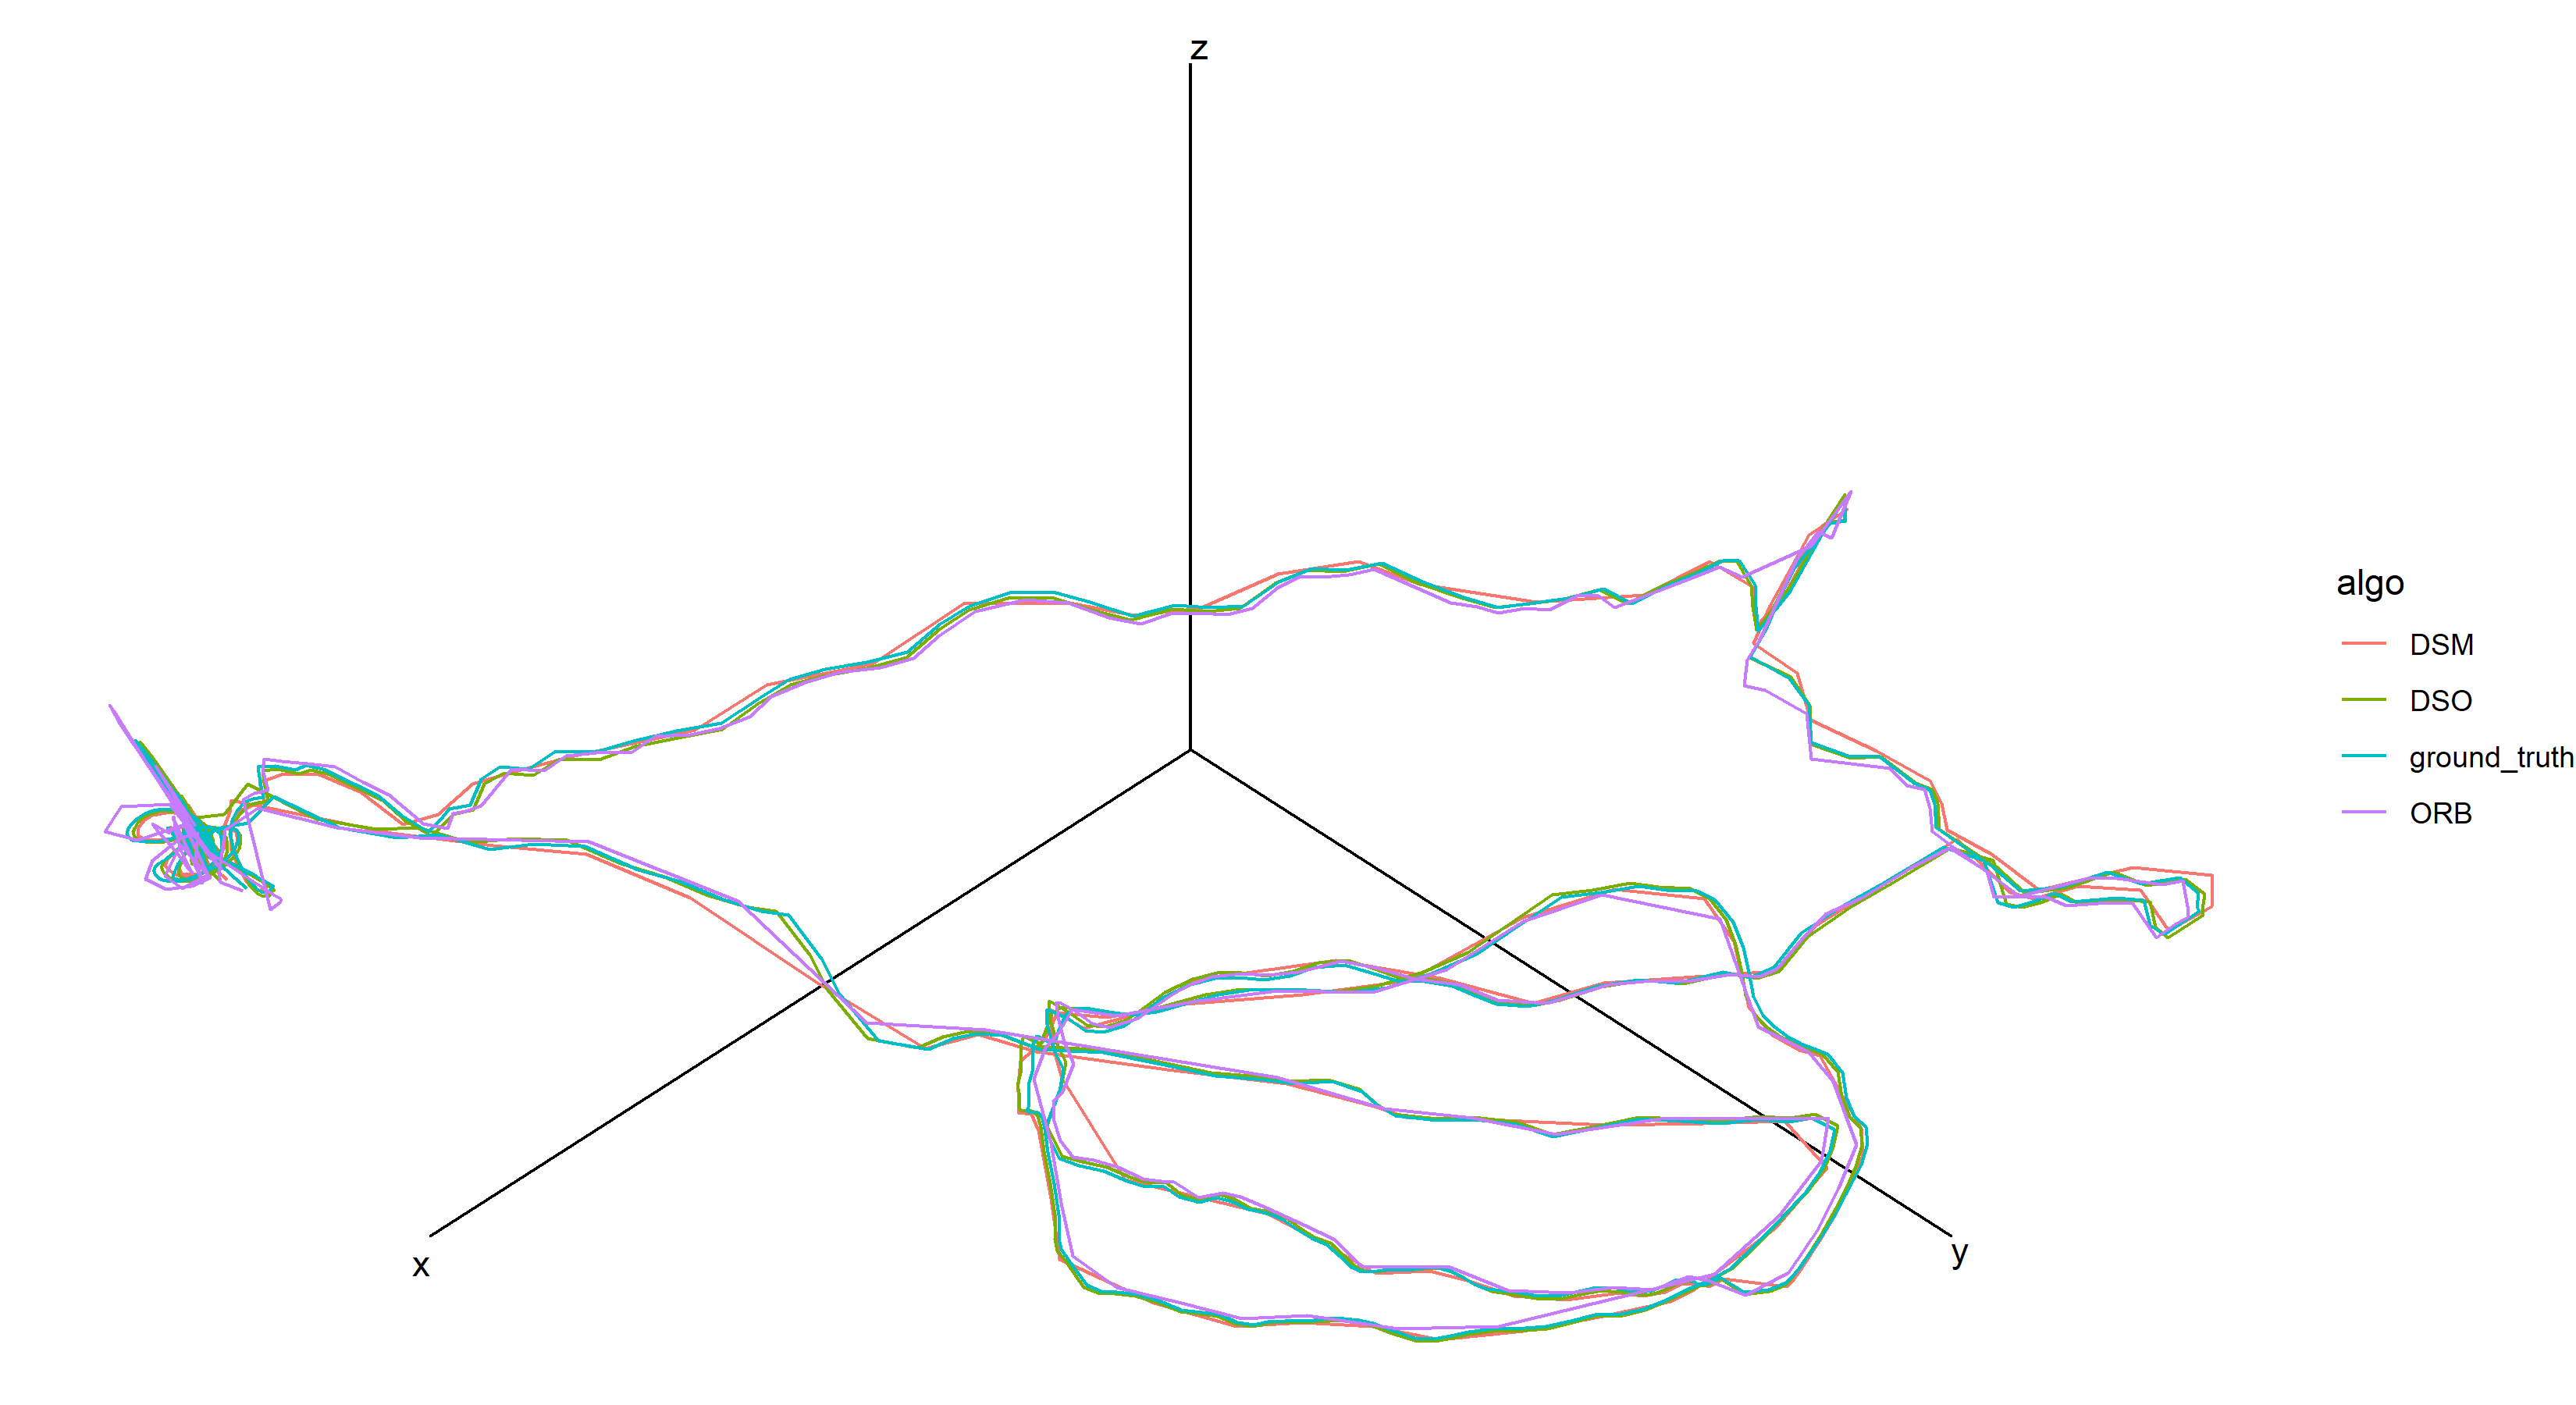
\includegraphics[width=9cm]{img/traj_perf.png} }}%
    \qquad
    \subfloat[\centering V102]{{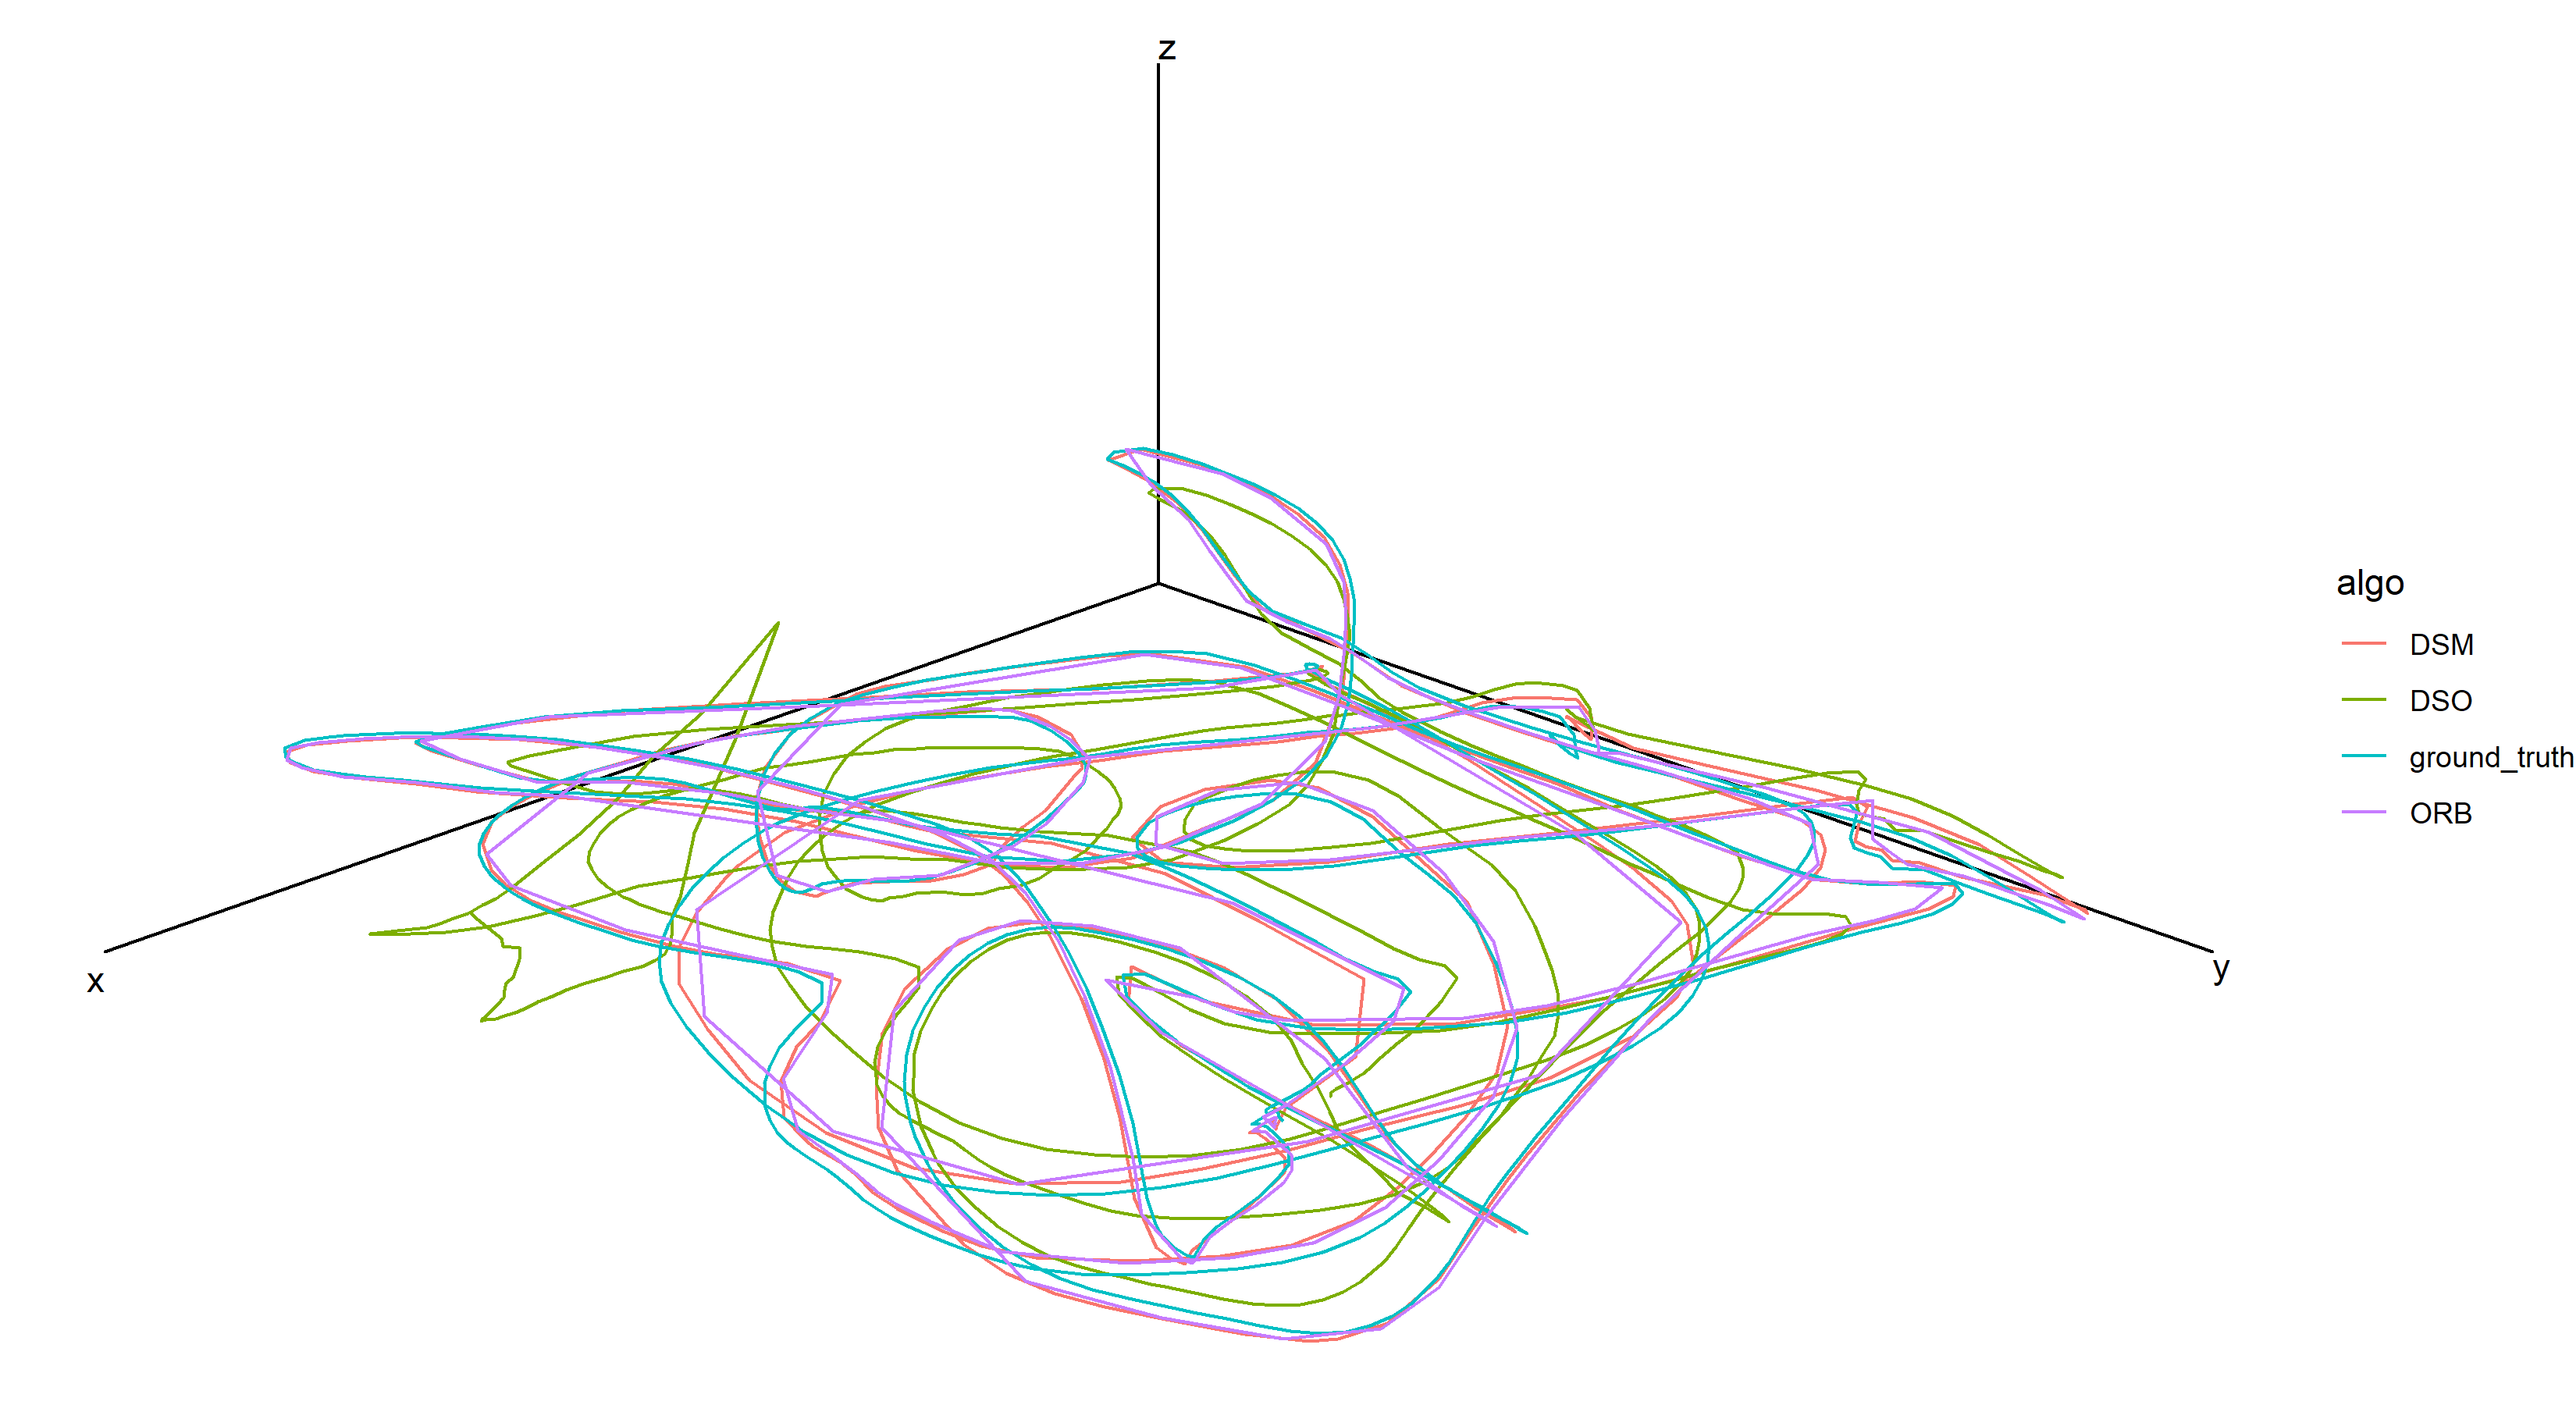
\includegraphics[width=9cm]{img/traj_dso.png} }}%
	\qquad
    \subfloat[\centering V203]{{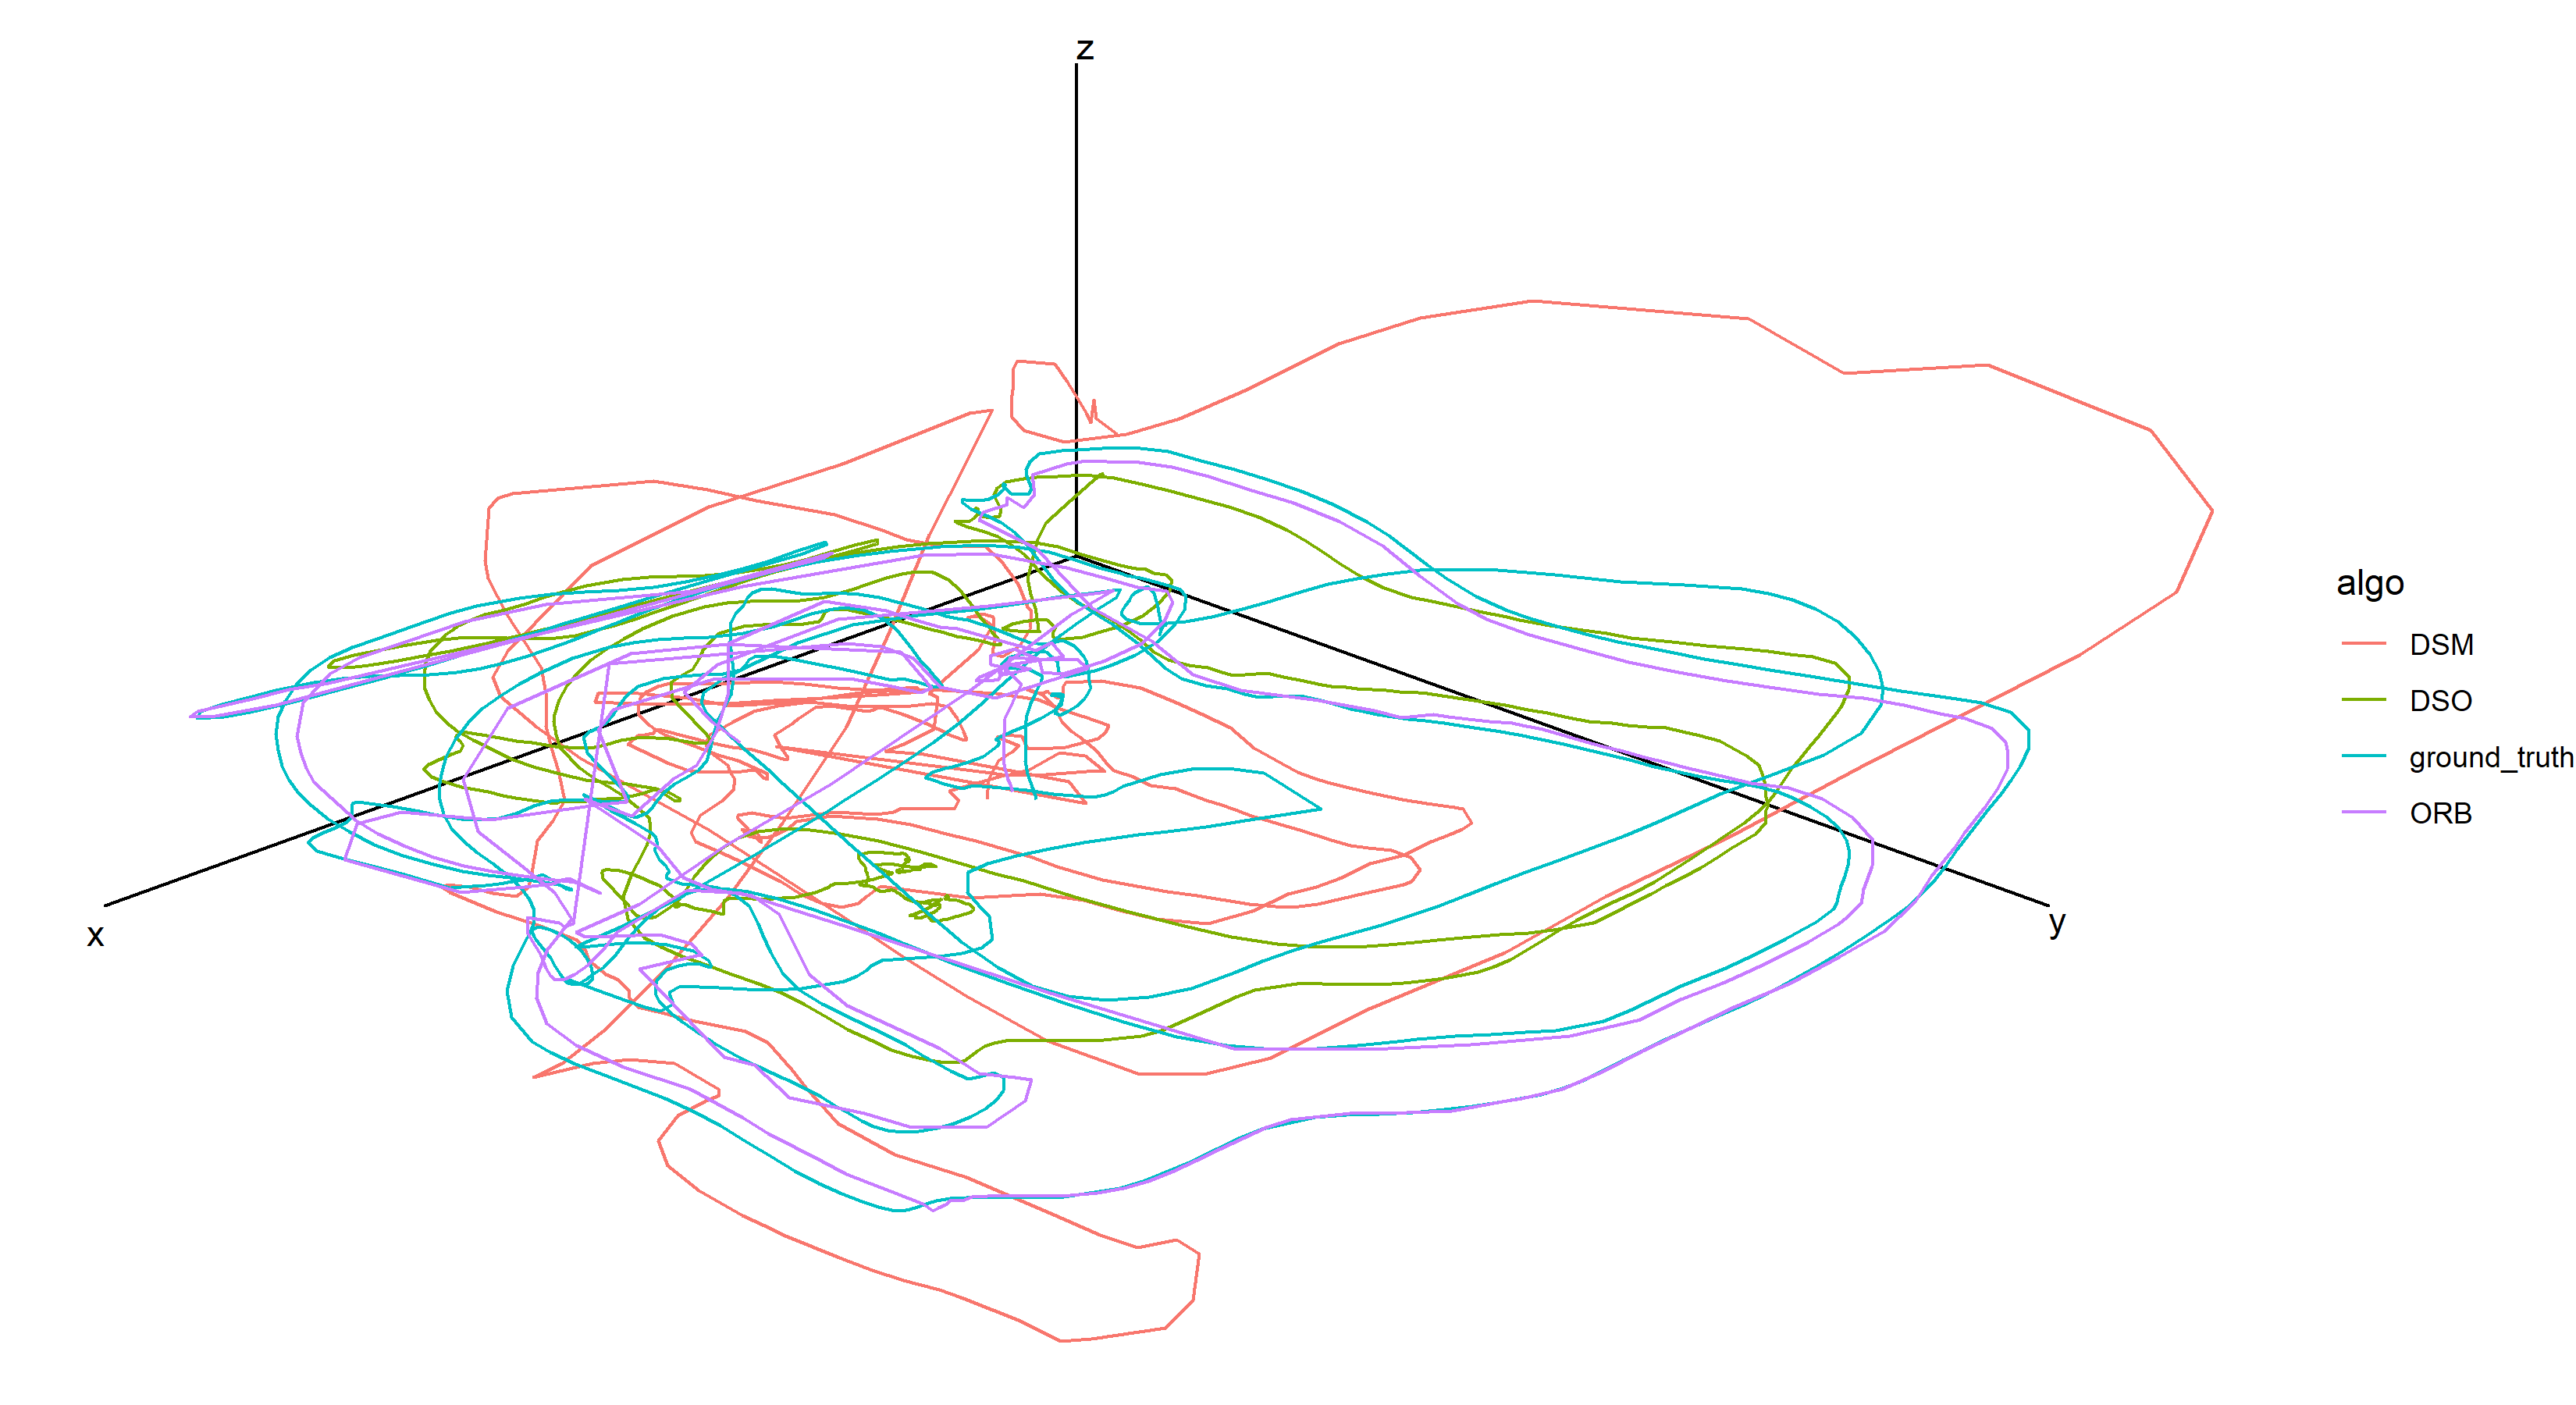
\includegraphics[width=9cm]{img/traj_last.png} }}%
    \caption{
	Ground truth flight path and evaluated flight path of each algorithm after alignment with the method of Umeyama in the x and y axis in meters. 
	Left the sequence MH01, middle the sequence V102 and right the sequence V203 is displayed.
	}%
    \label{fig:flight_path}%
	\end{figure}
	
	In figure \ref{fig:flight_path} the computed trajectories are plotted against the groundtruth for sequences MH01, V102 and V203 considering only the 
	x and y coordinate. These sequences 
	were selected, because they represent the results of the visual analalysis well. In the first sequence, MH01, all algorithms showed excellent results. 
	One reason for this could be, that in the first sequence, the camera only does very gentel movements, moving at an average speed of $0.41 ms^{-1}$. 
	
	The second image shows the sequence V102. Here, ORB and DSM show good results, since in most parts, the trajoctories are aligned perfectly. DSO on the 
	other hand shows a significant difference in the flight path. When observing the trajectory closely, the assumtion is raised, that the algorithm lost tracking 
	and therefore computed significant wrong postion data. This might have caused the calculated positions in the right of the plot, that have a large distance to 
	the groundtruth. The rest of the sequence might have been correctly estimated, however since the alignment is done minimzing \ref{sdfasdf}, one significant 
	mistake in the position estimation, might result in horrific results over the entire sequence after alignment. This is supported by watching the algorithm running
	and by the fact that in the plot, the trajectory looks very similar to the groundtruth, only with a significantly smaller scale.
	
	The last plot shows the results of the last sequence. Here, all algorithms had problems estimating a position that comes close to the groundtruth position. ORB
	SLAM still showed acceptable performance. 
	
	\fig{img/pos_error.png}{The positional error over time in meters. The vertical lines indicate the beginning of a new sequence}{fig:pos_error}{1}
	
	Furthermore, the eucleadian distances between position of the keyframe and the true postion of the latter are computed. For a keyframe, 
	the entry of the groundtruth data with the lowest distance in time to the time the keyframe was inserted is taken as reference point. 
	This is justifiable, since the true position is sampled at a frequency of over 200 points per second. 
	
	Figure \ref{fig:pos_error} shows these distances over time for all sequences and for all algorithms. As suspected, in the first five sequences in the machine 
	hall all algorithm performed good. The availability of more features in the scenery and the slow motions of the camera might explain the yielding of these results. 
	Also, it can be noticed, that DSO SLAM drifts further apart from the ground truth position with the continuety of the sequence in the sequences MH01, MH03 and V202. 
	This might be the result of lacking the functionality to close loops and to optimize over the global map, as explained in section \ref{asdfasdf}. 
	
	In figure \ref{fig:boxplot_traj} a boxplot of all computed distances over all sequences is displayed. This plot summarieses the results of the 
	trajectory analysis. The ORB algorithm, yielding a median positional error of 5.4 cm, performes slightly better than the DSO algorithm. DSO SLAM 
	shows inconsistent results with a median positional error of more than 10cm and a large amount of errors greater than half a meter. 
	
	\fig{img/boxplot_dist.png}{Boxplot of all euclideans distances between the ground truth position of the keyframe and 
	the evaluated position after alignment with the method of Umeyama. Outliers greater than 1.5 are not displayed for clarity reasons. 
	}{fig:boxplot_traj}{1}
	
	
\subsection{Pointcloud Evaluation}

For the evaluation of the computed point clouds, these point clouds were first visually observed, as described in section \ref{sec}. 
Figure \ref{fig:pointcloud} shows the evaluated point clouds aligned with the ground truth point cloud for sequence V101. This is a sequence, 
where the tracking of the trajectory was successfull for all three algorithms, thus, the errors of the resulting point clouds can not 
be a result of errors in alignment. 

What becomes clear at first glance is, that as mentioned, ORB generates only few points, since only found keypoints are mapped in feature based methods.
 To give these  points better visibilty, the point size was doubled in the ORB image. DSM and DSO slam generate point clouds with significant higher 
 density, where all structures of the room are clearly visible at first glance. 
 
 However, the advantace of ORB-SLAM over the other two direct methods 
 is the recognizing of clear features in terms of strucural differences in the scenes. Though, DSO and DSM also regard the differences in pixel intensities
 ORB, as described in section \ref{refasdf}, detects the features on different scale levels and ensures, that the regarded features are in fact significant. 
 This also became clear when observing the point cloud. All significant features, and therefore important features for autonomous navigation, were successfully 
 marked with a computed point. For example, this can be seen at the leiter?? in image three of figure \ref{fig:pointcloud}, where all sprossen contain at least 
 one point. 
 
 After closely observing the point clouds, it became clear, that the point clouds of DSO, often times generate point clouds, where multiple layers of 
 points were falsly generated, where all points had the same clear distance to the ground truth point cloud. This may be a result of working of DSO slam, 
 where keyframes, that are marginalized, are removed permanently. When revisiting areas, the points are again generated. This means that all errors made
 in the sequence accumulate and when an area is revisited, significant errors in the point cloud can be made. This can be seen when looking at the 
 third image closely. When looking at the matraccess in the middle of the room, the accumulated error expresses itself by points hovering in the air 
 in a clear plane. 
 
 % irgendwo noch das dynimaische umgebung problem für slam ist. 

	\begin{figure}%
    \centering
    \subfloat[\centering ORB]{{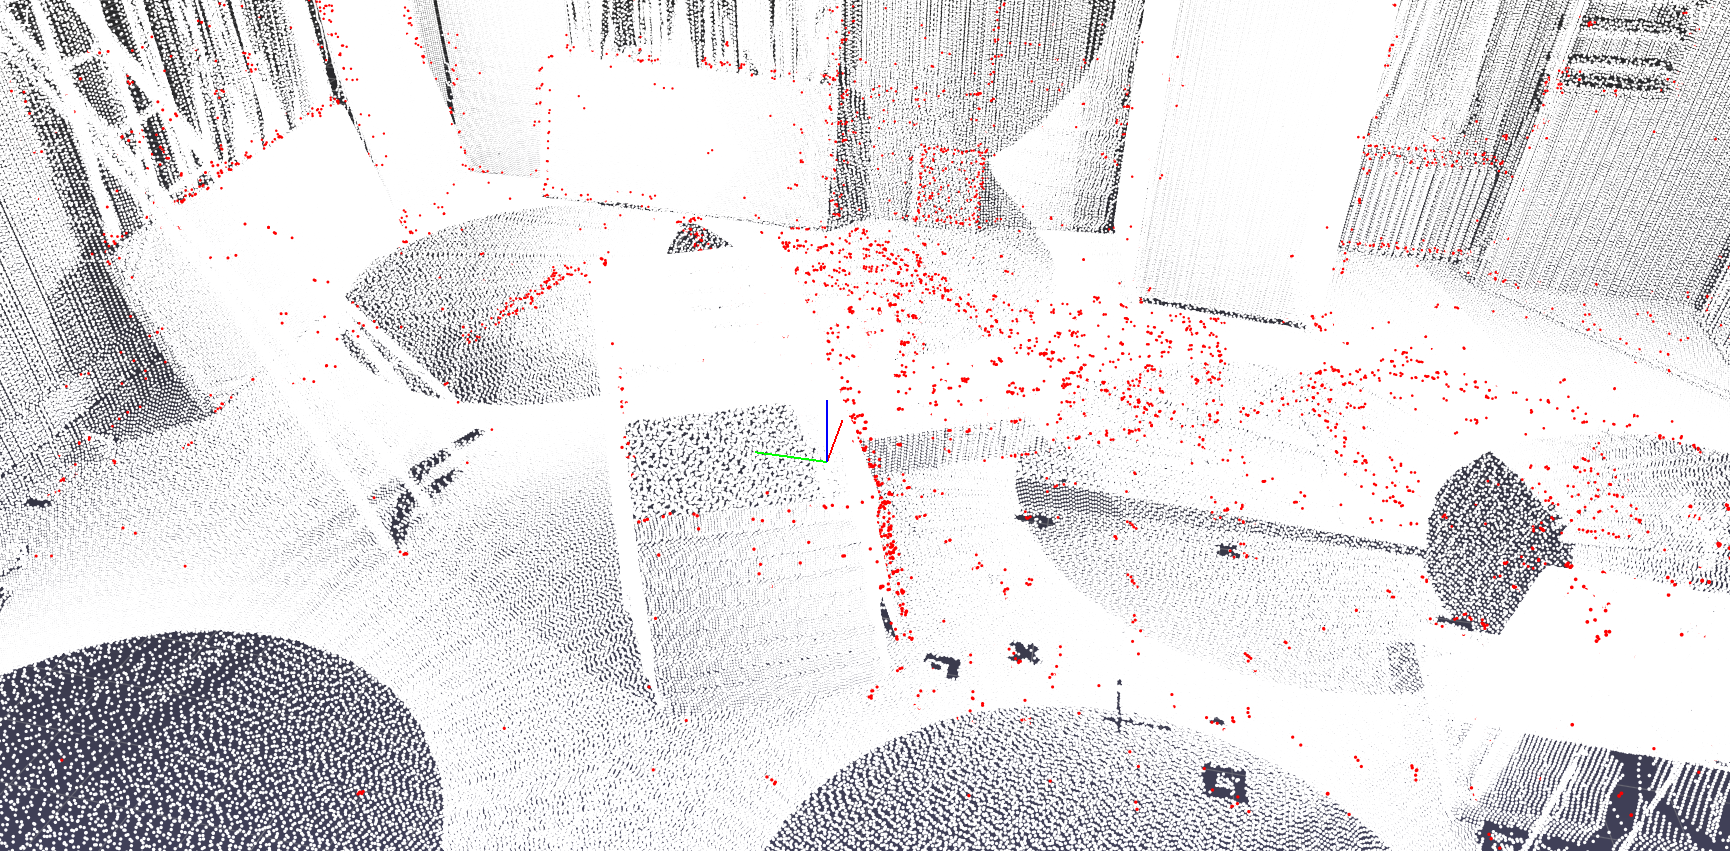
\includegraphics[width=7cm]{img/pointcloud_orb} }}%
    \qquad
    \subfloat[\centering DSM]{{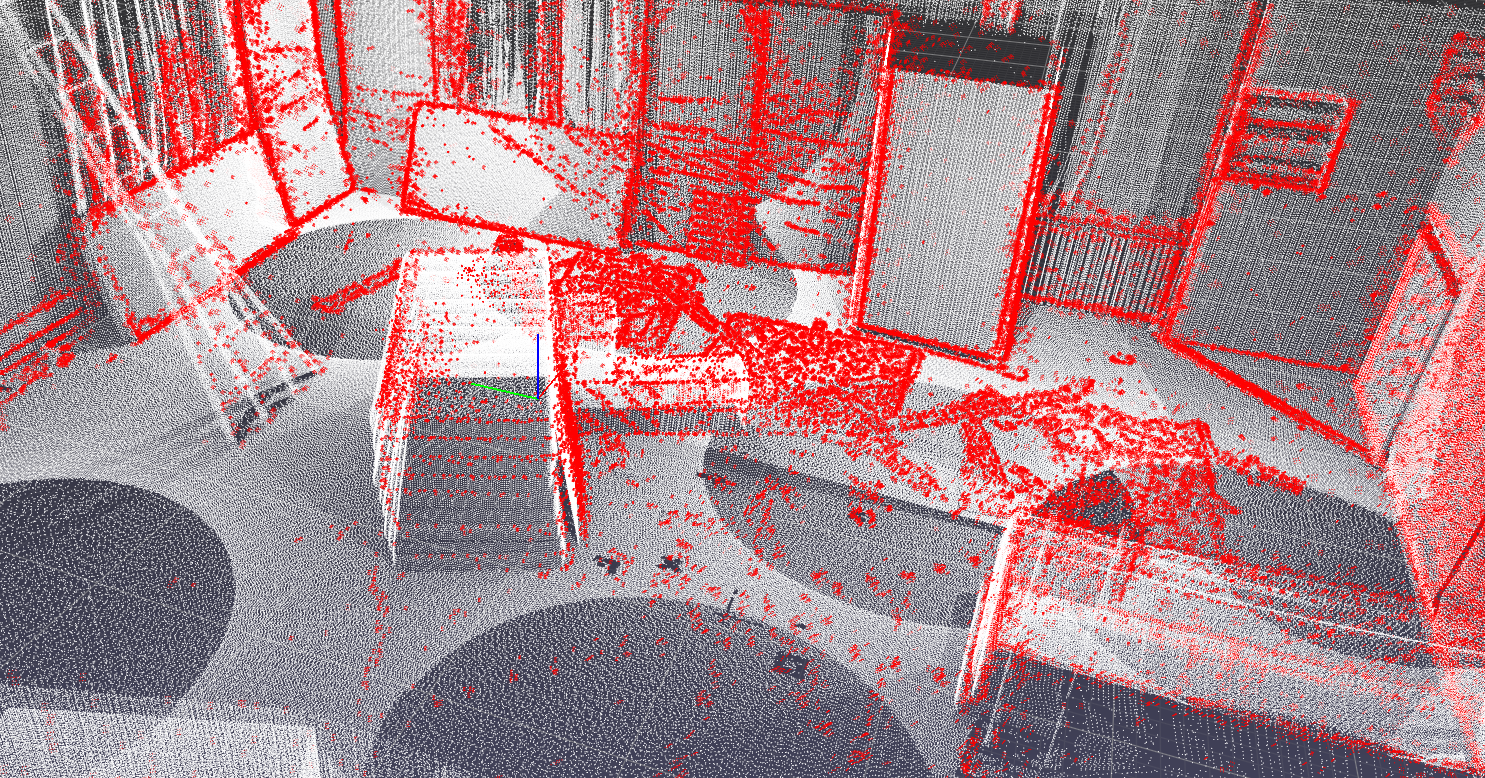
\includegraphics[width=7cm]{img/pointcloud_dsm} }}%
	\qquad
    \subfloat[\centering DSO]{{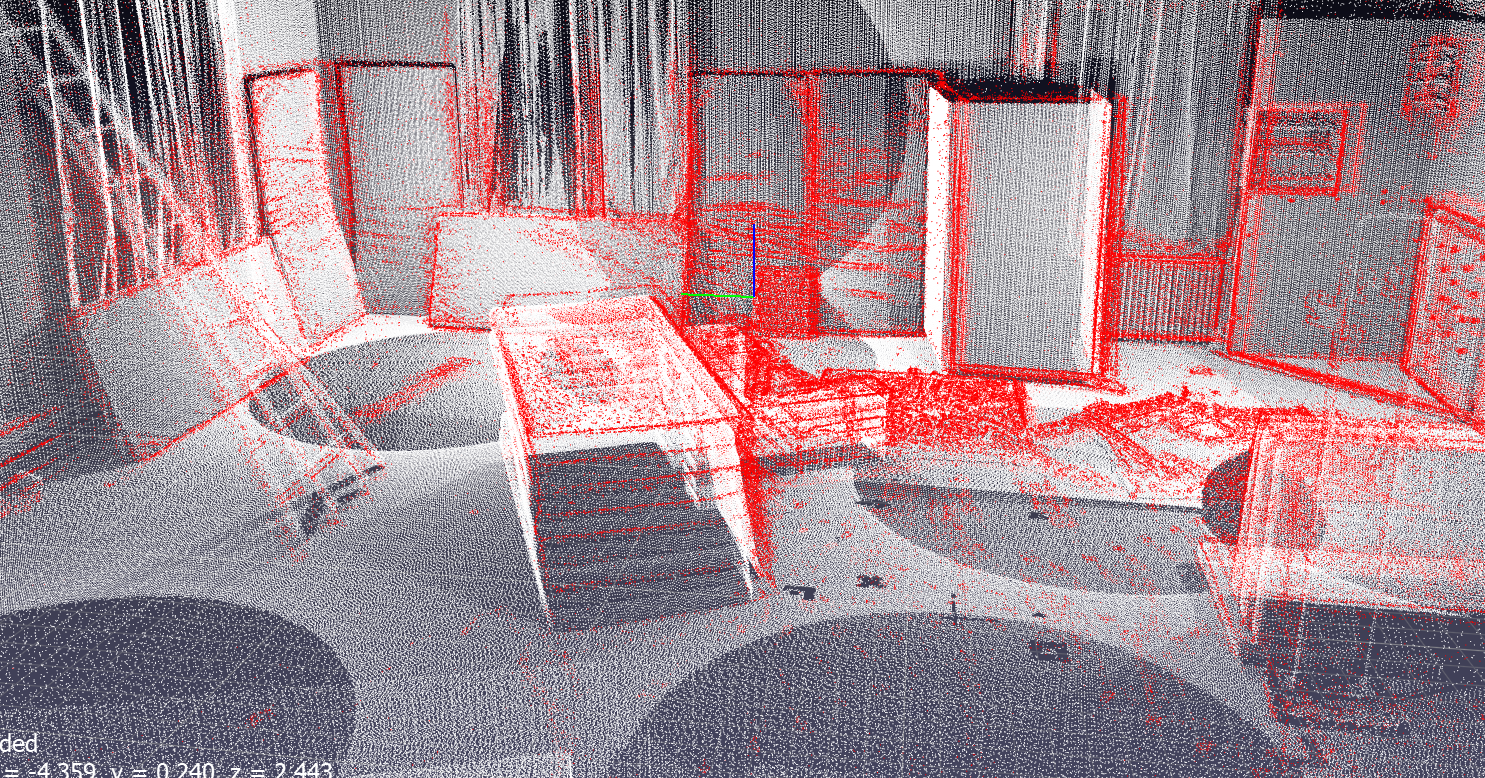
\includegraphics[width=7cm]{img/pointcloud_dso} }}%
    \caption{The ground truth of the point cloud from Sequence V101 (white points) and the evaluated points by each algorithm (red points). 
	The points in Figure (a) are twice as large for better visibility (ORB-SLAM generates only few points). 
	}%
    \label{fig:pointcloud}%
	\end{figure}
	
	
	The density can also be expressed by numbers. The significant difference of the numbers of points can be seen in table \ref{table:pointcloud}. While 
	ORB slam only generates close to 10000 points in the sequences DSM slam generates more than 500000 points in most sequences and DSO more than 200000 
	in most sequences. 
	
	\begin{table}
	\caption{Absolute number of points and distance to closest point in the ground truth point cloud in meter for each algorithm and sequence.}
	\begin{tabular}{ |p{3cm}||p{3cm}|p{3cm}|p{3cm}|  }
	\hline
	Sequence Name& ORB & DSM & DSO \\
	\hline
	MH\_01\_easy & 8958 (/) & 675720 (/) & 361633 (/)\\
	MH\_02\_easy & 8692 (/) & 700920 (/) & 343804 (/)\\
	MH\_03\_medium & 7445 (/) & 614264 (/) & 371752 (/)\\
	MH\_04\_difficult & 7943 (/) & 495752 (/) & 208445 (/)\\
	MH\_05\_difficult & 8373 (/) & 517712 (/) & 232415 (/)\\
	V1\_01\_easy & 7075 (0.049) & 6108440 (0.066) & 374257 (0.066)\\
	V1\_02\_medium & 6517 (0.042) & 648440 (0.187) & 366513 (1.458)\\
	V1\_03\_difficult & 7983 (0.052) & 775080 (0.092) & 448212 (0.459)\\
	V2\_01\_easy & 5688 (0.049) & 584552 (0.58) & 247905 (0.086)\\
	V2\_02\_medium & 8129 (0.074)& 733992 (0.078) & 490608 (0.104)\\
	V2\_03\_difficult & 7359 (0.17) & 921312 (0.645) & 465396 (0.677)\\
	\hline
	\end{tabular}
	\label{table:pointcloud}
	\end{table}
	
	However, regarding the accuracy of the computed points by the algorithms, again ORB-SLAM shows the best performance. In table \ref{table:pointcloud}, 
	for all sequences, where a groundtruth pointcloud exists, the distance to the closest point in the groundtruth point cloud is computed by randomly sampling
	500 points per algorithm and sequence. In all except the last, ORB-SLAM yields a mean distance of less than 10cm while DSM and DSO SLAM also yield results 
	greater than 50 cm for certain sequences. 
	
	
	\fig{img/pq_dist.png}{Boxplot of the euclidean distances between an evaluated point and the closest point of the ground truth point cloud.
	For computational feasibility, for each sequence and algorithm, 500 points for evaluation are sampled randomly}{fig:boxplot_pq}{1}
	
	

\subsection{Calculation Time}

	For each sequence and algorithms, the computational time was taken, that the algorithm took, to complete the computation of the sequence. 
	The time needed for initialization was not considered for the absolut time. 
	
	In order to evaluate, if an algorithm can run in realtime, the absolut times have to be broken down into the computed frames per second.
	The euroc dataset consists of sequences recorded at a frame frequence of 20 frames per second. This means the total frames per sequence 
	are amount to duration\_of\_sequence x 20. For the computed frames per second, this value is then devided by the time the algorithm needed 
	to process the sequence. 
	
	It is possible to decrease the frame 
	frequence, but this will also increase the risk of loosing the tracking, since the steps between the frames are greater and 
	the ??foreward motion model?? cannot pridict the new position as well für einen gewissen algo. % quelle
	
	The results are displayed in table \ref{table:comp_time}. ORB-SLAM processes the frames at a frame per second rate ranging from 11,1 (V102) to 16,1 (V203), 
	DSM SLAM processes the frames at a range from 0,9 (V103) to 3,3 (MH01) frames per second and DSO slam at a rate in range of 1,5 (V202) to 4,9 (MH01). Thus, 
	none of the evaluated slam algorithms processes any of the evaluated sequences in realtime. 
	
	% DSO enforce realtime not working

	\begin{table}
	\caption{Computation time (excluded time needed for initialization) of each sequence and algorithm. In parentheses the 
	resulting computed frames per second are given.}
	\begin{tabular}{ |p{3cm}||p{3cm}|p{3cm}|p{3cm}|  }
	\hline
	Sequence Name & Computation Time in $s$ ORB & Computation Time in $s$ DSM & Computation Time in $s$ DSO \\
	\hline
	MH\_01\_easy & 257 (14,2) & 1098 (3,3) & 749 (4,9)\\
	MH\_02\_easy & 209 (14,4) & 984 (3,1) & 690 (4,4)\\
	MH\_03\_medium & 198 (13,3) & 1369 (1,9) & 707 (3,7)\\
	MH\_04\_difficult & 165 (12) & 896 (2,2) & 504 (3,9)\\
	MH\_05\_difficult & 193 (11,5) & 825 (2,7) & 633 (3,5)\\
	V1\_01\_easy & 253 (11,4) & 1383 (2,1) & 905 (3,2)\\
	V1\_02\_medium & 150 (11,1) & 1550 (1,1) & 820 (2,0)\\
	V1\_03\_difficult & 186 (11,3) & 2262 (0,9) & 1134 (1,9)\\
	V2\_01\_easy & 187 (12) & 1045 (2,1) & 612 (3,7)\\
	V2\_02\_medium & 162 (14,2) & 1675 (1,4) & 1522 (1,5)\\
	V2\_03\_difficult & 143 (16,1) & 1600 (1,4) & 793 (2,9)\\
	\hline
	\end{tabular}
	\label{table:comp_time}
	\end{table}

